\label{referencial}

Neste Capítulo apresentamos ...

\section{Engenharia de Software}
 Engenharia de software é o processo que foca nas áreas de planejamento, desenvolvimento e entrega dos sistemas de software. É com este tipo de metodologia que conseguimos estimar de maneira mais apurada formas de como desenvolver o sistema, estimar prazos, recursos e até mesmo espaços para melhora durante e após a conclusão do projeto. A engenharia de software nasceu da necessidade de entregar ao cliente uma maior garantia de qualidade, sem deixar de lado a preocupação com prazos, estes cada vez mais curtos perante as demandas que o mundo e sua evolução tecnológica tem exigido \cite{DBLP:books/lib/Sommerville07}. 

\subsection{Engenharia de Requisitos}
A engenharia de requisitos (ou especificação de software) é a área responsável por entender e decidir quais serão as requisições necessárias ao sistema solictado e verificar os impedimentos relacionados ao desenvolvimento e operação do sistema. Costuma ser um estágio crítico do processo de criação de um software, pois uma vez mal desenhado e com erros nesta fase, mais a frente no projeto, implantação e manutenção do sistema problemas serão comuns de aparecerem \cite{Sommerville07}.

Esta etapa existe com o propósito de criar uma documentação de requisitos acordados onde cria a especificação de um sistema que possa atender às necessidades dos clientes atendidos para o desenvolvimento do software. Usualmente, os requisitos são postos para seus clientes e usuários finais em um nível mais alto, sem grandes detalhes técnicos, enquanto para os desenvolvedores é essencial que os detalhes técnicos sejam muito bem apresentados \cite{Sommerville07}.

De acordo Sommerville \cite{Sommerville07}, são quatro níveis principais do processo de engenharia de requisitos, que são os seguintes:
\begin{enumerate}
    \item \textit{Estudo de viabilidade}: Realiza-se uma aproximação a respeito a possibilidade de se cumprir com as requisições do usuário em questão, valendo-se de tecnologias contemporâneas, seja a nível de software ou de hardware. Esse estudo leva em conta se o sistema a ser criado será lucrativo sobre uma posição de negócio e se o mesmo pode ser construído sob condições financeiras limitadas. Um estudo de viabilidade deve ser algo sem grandes custos e de rápida conclusão, onde o resultado culmina na decisão ou não de continuar com a possibilidade de um estudo mais detalhado.
    \item \textit{Elicitação e análise de requisitos}: Esta é a parte do processo onde se inicia a formação mais aprofundada dos requisitos do sistema por meio da análise de outros sistemas existentes, além de debates com os potenciais clientes/usuários e compradores, verificação de tarefas e outras etapas. É nesta parte onde a criação de protótipos ou modelos de sistemas são feitos para ajudar a elucidar o sistema a ser criado.
    \item \textit{Especificação de requisitos}: A etapa de ação de tradução dos dados e informações coletados durante a etapa de análise de uma documentação que detalha o connjunto de requisitos. Geralmente, são dois os tipos de requisitos que podem ser inseridos nesta documentação. A parte onde o cliente fala o que deseja criar para o seu produto de forma mais geral e sem a profundidade técnica, mais voltada para o objeto de desejo de uso é chamada de requisitos de usuário, enquanto a parte onde há um maior detalhamento na descrição técnica a ser fornecido ao usuário é chamado de requisitos de sistema.
    \item \textit{Validação de requisitos}: Esta etapa é onde verificamos se o sistema está consistente, completo e de acordo com a realidade, onde não por acaso se descobrem os principais erros e a documentação deve ser alterada de forma a visar a correção destes problemas que foram mapeados durante esta etapa.
\end{enumerate}

\begin{figure}
    \centering
    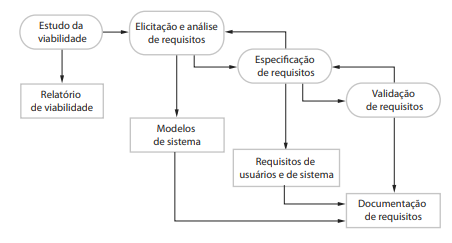
\includegraphics{img/eng_req.png}
    \caption{Gráfico do processo de engenharia de requisitos} \cite{Sommerville07}
    \label{fig:eng_req}
\end{figure}


\section{Desenvolvimento Ágil de Software}

\subsection{Scrum}

\subsection{Planning Poker}

\section{Inteligência Artificial}

\subsection{Ética em IA}


\section{Trabalhos Relacionados}
